\documentclass{article}
\usepackage[utf8]{inputenc}

\title{Strong capacitive interactions within the non-equilibrium Green's Function Formalism.}
\author{Josko de Boer}
\date{December 2016}
\usepackage[square,numbers]{natbib}
\bibliographystyle{abbrvnat}
\usepackage{fourier}
\usepackage{multicol}
\usepackage{fullpage}
\usepackage[british]{babel} 
\usepackage{mathrsfs}
\usepackage{amsthm,amsmath,amssymb,amsfonts}  
\usepackage{braket} 
\usepackage{subcaption}
\usepackage{xcolor}
\usepackage{graphicx}
\renewcommand{\thefootnote}{\Roman{footnote}}
\newcommand{\red}[1]{ {\color{red} #1}}
\date{February 2017}

\begin{document}
\maketitle
\begin{abstract}
    Most work on interactions for molecular junctions have been performed within the Master equation approach. This approach has the benefit of incorporating vibrational excitations and interactions up to desired order. In this work we focus on the non-equilibrium Green's function formalism. We incorporate interactions and derive the many-body Green's function. The density matrix emerges as a self-consistent equation that is in principle exactly solvable. We first apply these principles to the case of a coulomb Island, a much studied and discussed nanoscopic device.  Having established both the basics and the Kondo physics of this device, we move on to consider the intrinsic and pronounced NDC effect in a single thiolated arylethynylene molecule with a 9,10-dihydroanthracene. We show that incorporation of strong capacitive interaction greatly improves the agreement between theory and experiment. The new theory has exciting promise for future studies of molecular junctions.
\end{abstract}
\begin{multicols}{2}
    
    \section{Introduction}
        One of the challenges for the theory of molecular junction devices has always been to incorporate the details of specific molecules. One popular approach is to solve the Kohnn-Sham equations\cite{kohnsham}, which reformulate the many-body Schr\"dinger equation in terms of the electron density $n(\underline{r})=\sum_{\sigma,i}\:n_{\sigma i}(r)$. This is called Density-Functional theory (DFT) \cite{nobel1998}, which leads to the single-particle Hamiltonian of a specific molecule.  
        
        If vibrational modes are of interest then the transport calculations are often done using the Master Equation (ME) approach \cite{beenakker}. The alternative is the non-equilibrium Green's function formalism (GF) approach. Both approaches struggle with accounting for strong interactions, which is is true of theoretical physics in general. 
        
        The method outlined here will incorporate strong \emph{capactive} interactions in the GF approach. It will emphasise the many-body character of the system and reconcile theory and experiment.
        
        We will first derive and introduce the theory in section~\ref{sec:derivation}. To illustrate the effectiveness and completeness of the effect we will look at the Coulomb Island model in section~\ref{sec:island}. For a far more interesting example, in section~\ref{sec:ahmolecule} we look at the Non-Differential Conductance (NDC) effect in a single thiolated arylethynylene molecule (AH molecule) with a 9,10-dihydroanthracene core, where the theoretical and experimental current have been found to match qualitatively but not quantitatively \cite{perrinnano}. Finally, we discuss the findings of our theory and its future promises in section~\ref{sec:discussion}.
    
    \section{Derivation}\label{sec:derivation}
        Let us start with clearly defining the Anderson-like model:
        \begin{align}
            H &= H_1 + H_2 + H_\tau + H', \label{eq:hamiltonian}
        \end{align}
        where
        \begin{align*}
        H_1 &= \sum_i \epsilon_i \hat{d_i}^\dagger \hat{d_i} + \sum_k E_k \hat{c_k}^\dagger \hat{c_k}, \\
        H_2 &= \sum_{ki}\left\{ V_{ki} \hat{c_k}^\dagger \hat{d_i} +  V_{ki}^\dagger \hat{d_i}^\dagger \hat{c_k} \right\},\\
        H' &= \frac{1}{2} \sum_{ij} U_{ij} \hat{n_i}^\dagger \hat{n_j},\\
        H_\tau &= \sum_{ij} \tau_{ij} \hat{d}_i^\dagger \hat{d}_j
        \end{align*}
        in which the creation (annihilation) operators $\hat{d_i}^\dagger, \hat{d_i}$ denote electrons on the region of interest, whereas the creation (annihilation) operators $\hat{c_k}^\dagger, \hat{c_k}$ denote electrons on the contacts. The Hamiltonian $H_2$ describes contact-lead coupling, while the interaction Hamiltonian $H'$ describes capacitive interactions in the device.
        
        The capacitive interactions are two-particle interactions under the assumption that they do not mix the eigenstates of the unperturbed Hamiltonian. In other words, removing an electron is assumed to change only the energy of the other electrons but not their spatial distribution. Naturally, self-interaction is not included ( $U_{ij} = U_{ij} (1-\delta_{ij})$) and is symmetric ($U_{ij} = U_{ji}$).
        
        For a derivation using the equation of motion method, we need to find the commutator of $H'$ with $\hat{d_i}$:
        \begin{align}
            \left[\hat{d_i}, H'\right] &= \sum_j U^j_{ij} \hat{n_j}\hat{d_j}, \label{eq:commutator}
        \end{align}
        where
        \begin{align*}
        U^k_{ij} &= U_{ij}^k \delta_{kj}
        \end{align*}
        is introduced to simplify future expressions. The equation of motion in the energy-domain is then found as:
        \begin{align*}
        \epsilon \hat{G}_{ij}^\pm &= \delta_{ij} + \epsilon_i \hat{G}_{ij}^\pm + \sum_k \tau_{ik} \hat{G}_{kj}^\pm + \sum_k U^k_{ik} \hat{n_k} \hat{G}_{ij}^\pm.
        \end{align*}
        Note that the final term leads to a capacitive self-energy $\hat{\Sigma}^c \equiv \sum_k U^k \hat{n_k}$ upon comparison with the Dyson equation. However, the capacitive self-energy is not yet in matrix form. The Coulomb Island example will show how to find the matrix form and final formalism.
        
        The Coulomb island is a simple example of our theory. It is a two-state system, with a singular level $\epsilon_0$ that allows for two spin-states under the Pauli exclusion principle. It is treated up to second order in \citet{haugjauho}, who point out that such calculations at finite bias had not been carried out at the time of writing. 
        
        For our treatment, we need to find the \red{Name} expansion of \red{operators}:
        \begin{align}
        \left[ \hat{A}^{-1} - \hat{B}\right]^{-1} &=\hat{A} + \hat{A}\hat{B}\hat{A} + \hat{A}\hat{B}\hat{A}\hat{B}\hat{A} + \ldots,
        \label{eq:expansion}\end{align}
        where in our case $\hat{A} = \hat{G^+}$, the single-particle Green's Function and $\hat{B}=\hat{\Sigma}^C$, the capacitive self-energy. We apply the expansion (equation~\ref{eq:expansion}) to the Coulomb Island single-particle Green's function:
        \begin{align*}
            \hat{G}^+(\epsilon) &= \left[ \begin{bmatrix} \epsilon - \epsilon_1 - \Sigma^\pm & \tau \\
\tau & \epsilon - \epsilon_2 - \Sigma^\pm \end{bmatrix}^{-1} - \begin{pmatrix} U n_\uparrow & 0 \\ 0 & U n_\downarrow \end{pmatrix} \right]^{-1} \\
            &= (1-\hat{n_\uparrow})(1-\hat{n_\downarrow}) \hat{A} + \hat{n_\uparrow} (1-\hat{n_\downarrow}) \left[ \hat{A}^{-1} - \hat{B}_1\right]^{-1} \\& + (1-\hat{n_\uparrow}) \hat{n_\downarrow} \left[ \hat{A}^{-1} - \hat{B}_2\right]^{-1} + \hat{n_\uparrow} \hat{n_\downarrow}, \left[\hat{A}^{-1} - \hat{B}_1 - \hat{B}_2 \right]^{-1}
        \end{align*}
        where we have gathered like products of number operators and have taken into account that $ n_\sigma^p = n_\sigma$ for occupation operators of a single spin-state.
        
        In general, we find:
        \begin{align}
        G^\pm(\epsilon) &= \left[ \epsilon - \hat{H}^\cdot - \hat{H_\tau} -\hat{\Sigma}^{\pm} - \Sigma^{C} \right]^{-1} \nonumber\\
        &= \sum_\kappa \left( \prod_{i\in\kappa} \prod_{j\notin\kappa} \hat{n}_i (1-\hat{n}_j) \right) \left[ \epsilon - \hat{H}^\cdot - \hat{H_\tau} - \sum_{i \in \kappa}U^i - \hat{\Sigma}^\pm \right]^{-1} \nonumber\\
        &= \sum_\kappa P_{\kappa\kappa} \left[\epsilon - \hat{H}^\cdot - \hat{H_\tau} - \sum_{i\in\kappa} U^i - \hat{\Sigma}^\pm \right]^{-1} \label{eq:grouping},
        \end{align} 
        where $\hat{H}^\cdot=\sum_i \epsilon_i \hat{d_i}^\dagger \hat{d_i}$ denotes the Hamiltonian for electrons on the molecule.
        
        Note that $P_{kk}$ is the diagonal of the probability operator, so that its expectation value is the diagonal of the reduced density matrix of the device. I want to discuss transport through a specific many-body state $\kappa$. Therefore, I define the many-body Green's Function as:
        \begin{align}
        \hat{\mathscr{G}}^{\kappa\pm}_{ij} (t,t') &= \mp \frac{\imath}{\hbar} \theta(\pm(t-t'))\left\{ \hat{n}_\kappa \hat{d}_i(t), \hat{d}_j^\dagger (t')\right\},
        \label{eq:mbgfdef}
        \end{align}
        where we have included the generalised number operator $\hat{n}_\kappa = \prod_{i\in\kappa} \hat{n}_i$. We can find the commutator of $\hat{n}_i$ with the lead-molecule Hamiltonian $\hat{H}_2$ and the tunnelling Hamiltonian $\hat{H}_\tau$, which is nonzero. It therefore prevents us from obtaining a closed expression for the many-body Green's function in matrix form. To continue, we assume that $\left[ n_i, H' + H_\tau \right]=0$, which is equivalent to cutting off tunnel couplings after first order. We can then find the expectation value of the many-body Green's Function :
        \begin{align}               
        \mathscr{\hat{G}}^{\kappa\pm} &= \sum_{\lambda\lambda'} C_\lambda C^\star_{\lambda'} \braket{\lambda \left| \left[ \epsilon-\hat{H} - \hat{\Sigma}^c - \hat{\Sigma}^\pm\right]^{-1} n_\kappa \right| \lambda'} \nonumber \\
        &= \sum_{\lambda\supseteq\kappa} P_{\lambda\lambda} G^{\lambda\pm},\label{eq:mbgfresult}
        \end{align}
        where $G^{\lambda\pm}$ denotes the single-particle Green's function in the many-body state $\lambda$:
        \begin{align*}
        \hat{G}^{\lambda\pm} &= \left[\epsilon - \hat{\mu}^\lambda - \hat{H}_\tau - \hat{\Sigma}^\pm \right]^{-1},
        \end{align*}
        in which
        \begin{align}
        \hat{\mu}^\lambda_{ij} &= \delta_{ij} \left( \hat{H} + \sum_{p\in\lambda} U_{ip} \right) \label{eq:result},
        \end{align}
        in which $\hat{H}^\kappa = \hat{\mu}^\kappa + \hat{H}_\tau$ is recognised as the effective single-particle Hamiltonian of the system in the many-body state $\kappa$. This can be directly obtained from DFT calculations. This is a very useful fact, as some molecules are hard to capture otherwise. In particular, \emph{many} DFT calculations together can be used to obtain (a good approximation of) the full shape of $\hat{H}^\kappa$, leading to a more complete description of transport through the formulae derived above. In particular the formalism should be more accurate for excitations, and explains Coulomb blockades. This is a useful result for molecules that aren't accurately described as a set of weakly coupled moieties.
        
        Nevertheless,we still have to consider the problem of determining the density matrix. First, recall the single-particle state occupation numbers:
        \begin{align*}
            \braket{\hat{n}_i} &= \sum_{\kappa: i\in \kappa} P_{\kappa\kappa},
        \end{align*}
        where the sum is over those many-body states $\ket{\kappa}=\left(\prod_{i\in\kappa}\hat{d}_i^\dagger \right)\ket{0}$ in which the single-particle state $\ket{i} = \hat{d}_i^\dagger \ket{0}$ is occupied. We can represent the the vector of occupation numbers by a matrix equation $\braket{\underline{n}} = KP$, where $P=\text{diag}(P_{\kappa\kappa})$ and $K$ is defined by:
        \begin{align}
            K_{i\beta} = \begin{cases} 1 & \quad i\&B=i, \\ 0 & \quad\text{otherwise}\end{cases},
        \label{eq:kmatrix}\end{align}
        where $\&$ is the binary \emph{and} operator. 
        The vector of occupation numbers can also be obtained from the (many-body) lesser Green's function at $t=t'$:
        \begin{align} 
            \braket{n_i} &= \sum_{\kappa: i \in \kappa} \braket{n_\kappa d_i^\dagger (t) d_i (t)} \nonumber\\ 
            &= \sum_{\kappa: i \in \kappa} \sum_{\lambda \supseteq \kappa} P_\lambda \int^\infty_{-\infty} \frac{d\epsilon}{2\pi\imath} \left(-G^{\lambda<}_{ii} (\epsilon)\right) \nonumber\\
            &= \sum_{\kappa: i \in \kappa} \sum_{\lambda \supseteq \kappa} P_\lambda \int^\infty_{-\infty} \frac{d\epsilon}{2\pi} \left[ \sum_\alpha f_\alpha(\epsilon) G^{\lambda+}(\epsilon) \Gamma^\alpha G^{\lambda-}(\epsilon)\right]_{ii} \nonumber\\ 
            &= \sum_\kappa W_{i\kappa} P_\kappa, \label{eq:wmatrix}
        \end{align}
        where the lesser self-energy is substituted from both the Keldysh equation~\cite{diventra} and the fluctuation-dissipation theorem~\cite{haugjauho}. Applying this theorem requires that the states are explicitly known for the many-body system, something that we have already assumed with not mixing eigenstates.       
        
        The matrix element $W_{i\beta}$ is defined as:
        \begin{align*}
        W_{i\beta} &= \sum_{\kappa: i \in \kappa} \Delta^\beta_\kappa \int^\infty_{-\infty} \frac{d\epsilon}{2\pi} \left[ \sum_\alpha f_\alpha(\epsilon) G^{\lambda+}(\epsilon) \Gamma^\alpha G^{\lambda-} (\epsilon)\right]_{ii},
        \end{align*} where $\Delta^\beta_\kappa$ ensures only those $\kappa$ that are in the superset of $\beta$ are counted. It is important to remember that the fluctuation-dissipation theorem specified the Fermi-Dirac distribution on the \emph{contacts}, thereby introducing finite bias as a relevant parameter for the density-matrix solution. We have found the following equations for $\braket{\underline{n}}$:
        \begin{align}
            \braket{\underline{n}} &= WP = KP\label{eq:selfconsistent},
        \end{align}
        where it cannot be guaranteed that the null-space of $W-K$ is one-dimensional. We could then use a self-consistent scheme to solve for $\braket{\underline{n}}$ starting from the equilibrium vector. This is conceptually similar to turning on the non-equilibrium interactions adiabatically, which could be interpreted as a variation of the Gell-Man-Low theorem\cite{gellmannlow, molinari}, yet is not because a self-consistent scheme cannot guarantee adiabatic steps.
        
        However, we must consider the implications of a null-space containing more than one vector. The physical quantity, $\braket{\underline{n}}$ is certainly unique. This implies that all vectors in the null-space result in the same value of the physical quantity. As a result, any vector in the null-space suffices to calculate the expectations of number occupation operators. This then immediately results in a unique green function which allows us to calculate transport properties of the equation.

    \section{The Coulomb Island}\label{sec:island}
        We are now ready to perform the calculations for a Coulomb Island. Following \citet{haugjauho}, we will set $\hat{H}_\tau = 0$. We need to be careful with the incorporation of the leads. In the penultimate step for equation~\ref{eq:wmatrix}, we note a summation over each lead due to the fluctuation-dissipation theorem. 
        
        For a two-state system (spin up, spin down) we find:
        \begin{align*}
            G^{\lambda<}_{ii}(\epsilon) &= \left(\left|G_{1i}(\epsilon)\right|^2 + \left|G_{i2}(\epsilon)\right|^2 \right)\left(f^L (\epsilon) \gamma^L+f^R (\epsilon) \gamma^R\right),
        \end{align*}
        where we have used that $(G^+)^\dagger=G^-$ and that the coupling is described by a diagonal matrix. Here, $\gamma^\alpha$ denotes the coupling strength to the left (right) contact $\alpha$.
        
        \begin{figure*}[b]
            \centering
            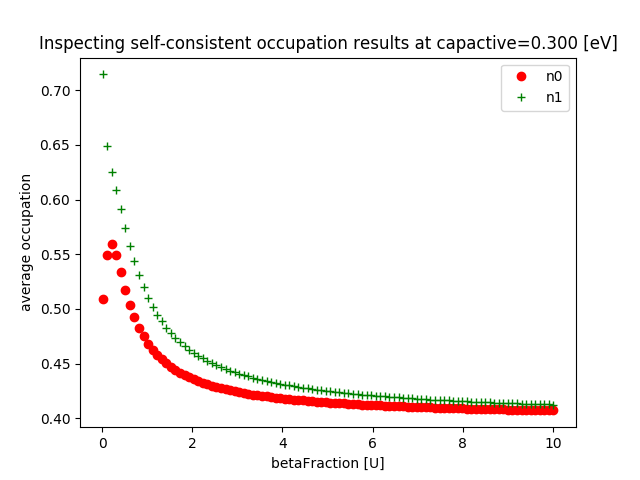
\includegraphics[width=\textwidth]{zeroBiasOccupation}
            \caption{\label{fig:numberoperators}Expectation value of occupation number operators $n_1$ and $n_2$.The emergence of a bound state at low temperatures is evident.}
        \end{figure*}
         
        
        In our calculation, the lead-molecule coupling (WBL) $\gamma=.010$ eV, the Coulomb repulsion $U=0.300$ eV, the first level is at $0.00$ eV and the second level at $0.030$ eV. We can immediately calculate the expectations of number operators, shown in fig~\ref{fig:numberoperators}.We observe the emergence of a bound state at low temperatures, evident in the exponential growth of $n_1$. In stark contrast, $n_0$ reaches its maximum and then rapidly falls off. Considering that we are dealing with the exact calculation of occupation for an Anderson-model, it is likely that we are observing evidence of the Kondo effect \cite{josherrereview}. This is typically evident in the conductance $\sigma(T)$, which decreases as a Fermi-liquid
        until reaching a conductance minimum at the Kondo temperature $T_K$, after which it logarithmically grows until saturating because of low-temperature screening effects.
        
        Following \citet{meir}, we look primarily at the conductance $\mathscr{T}(\epsilon)$ versus the chemical potential $\epsilon$. In a non-equilibrium situation the Fermi energy is rather badly defined; even more so in a mesoscopic region. The Fermi energy is a bulk property of the Fermi liquid model which does not hold in the extended molecule region. As such, we will consider the full conductance spectrum and follow the conductance maximum.
        
        Fig~\ref{fig:transplot} displays the differential conductance $T(\epsilon)$. Note the four peaks that are evidence of interaction effects for our two-state model. The differential conductance traces are offset by the temperature for reasons of clarity. A clear transition to zero-occupation is evident as the temperature grows. Of particular interest is the nonzero occupied state at low temperature, which is non-symmetric.
        
        \begin{figure*}[b]
            \centering
            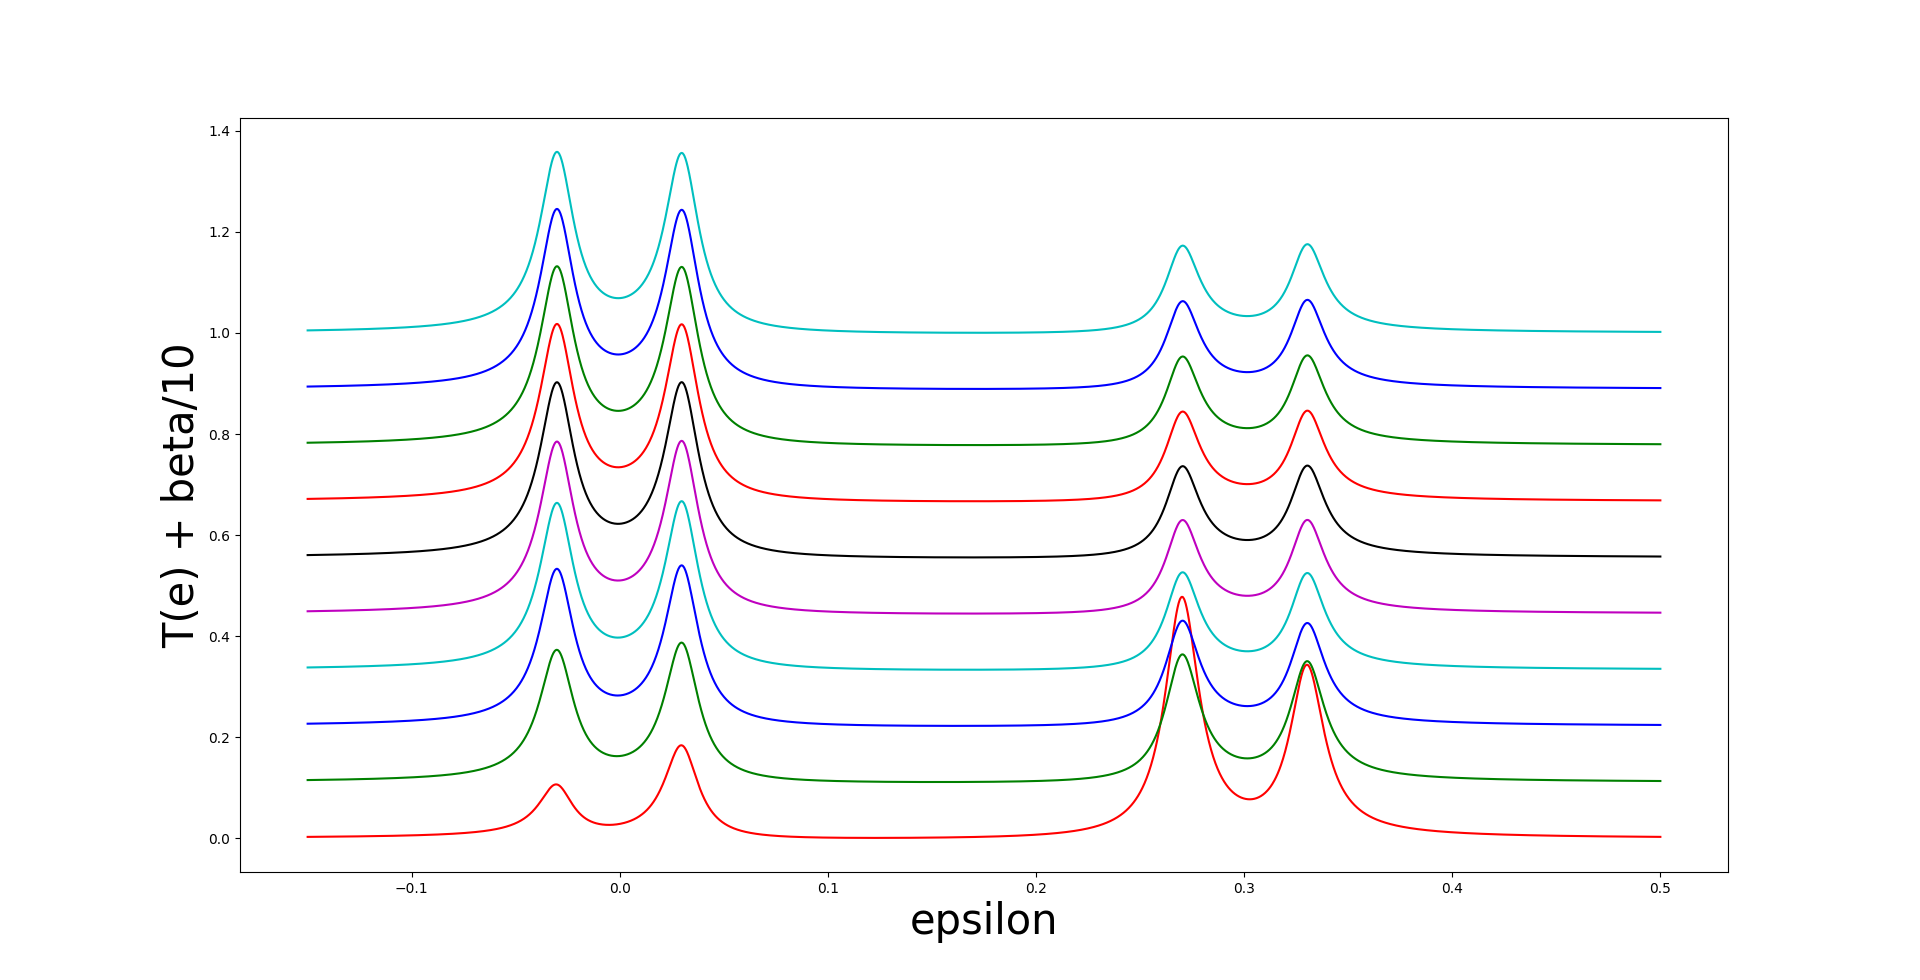
\includegraphics[width=\textwidth]{transportPlot}
            \caption{\label{fig:transplot} Differential conductance $T(\epsilon)$, displaying the multiple peaks that are evidence of interaction effects for our two-state model. The differential conductance traces are offset by the temperature for reasons of clarity. A clear transition to zero-occupation is evident as the temperature grows. Of particular interest is the nonzero occupied state at low temperature, which is non-symmetric.}
        \end{figure*}
        
        This state is clearly the bound-state that is responsible for the Kondo effect. Fig~\ref{fig:conductance} shows the average conductance {\color{red} We should probably follow the non-symmetric peak, so we can call it following the maximum.}, displaying clearly the polynomial decrease with temperature, followed by the conductance minimum, logarithmic rise and final screening saturation.
        
        \begin{figure*}[b]
            \centering
            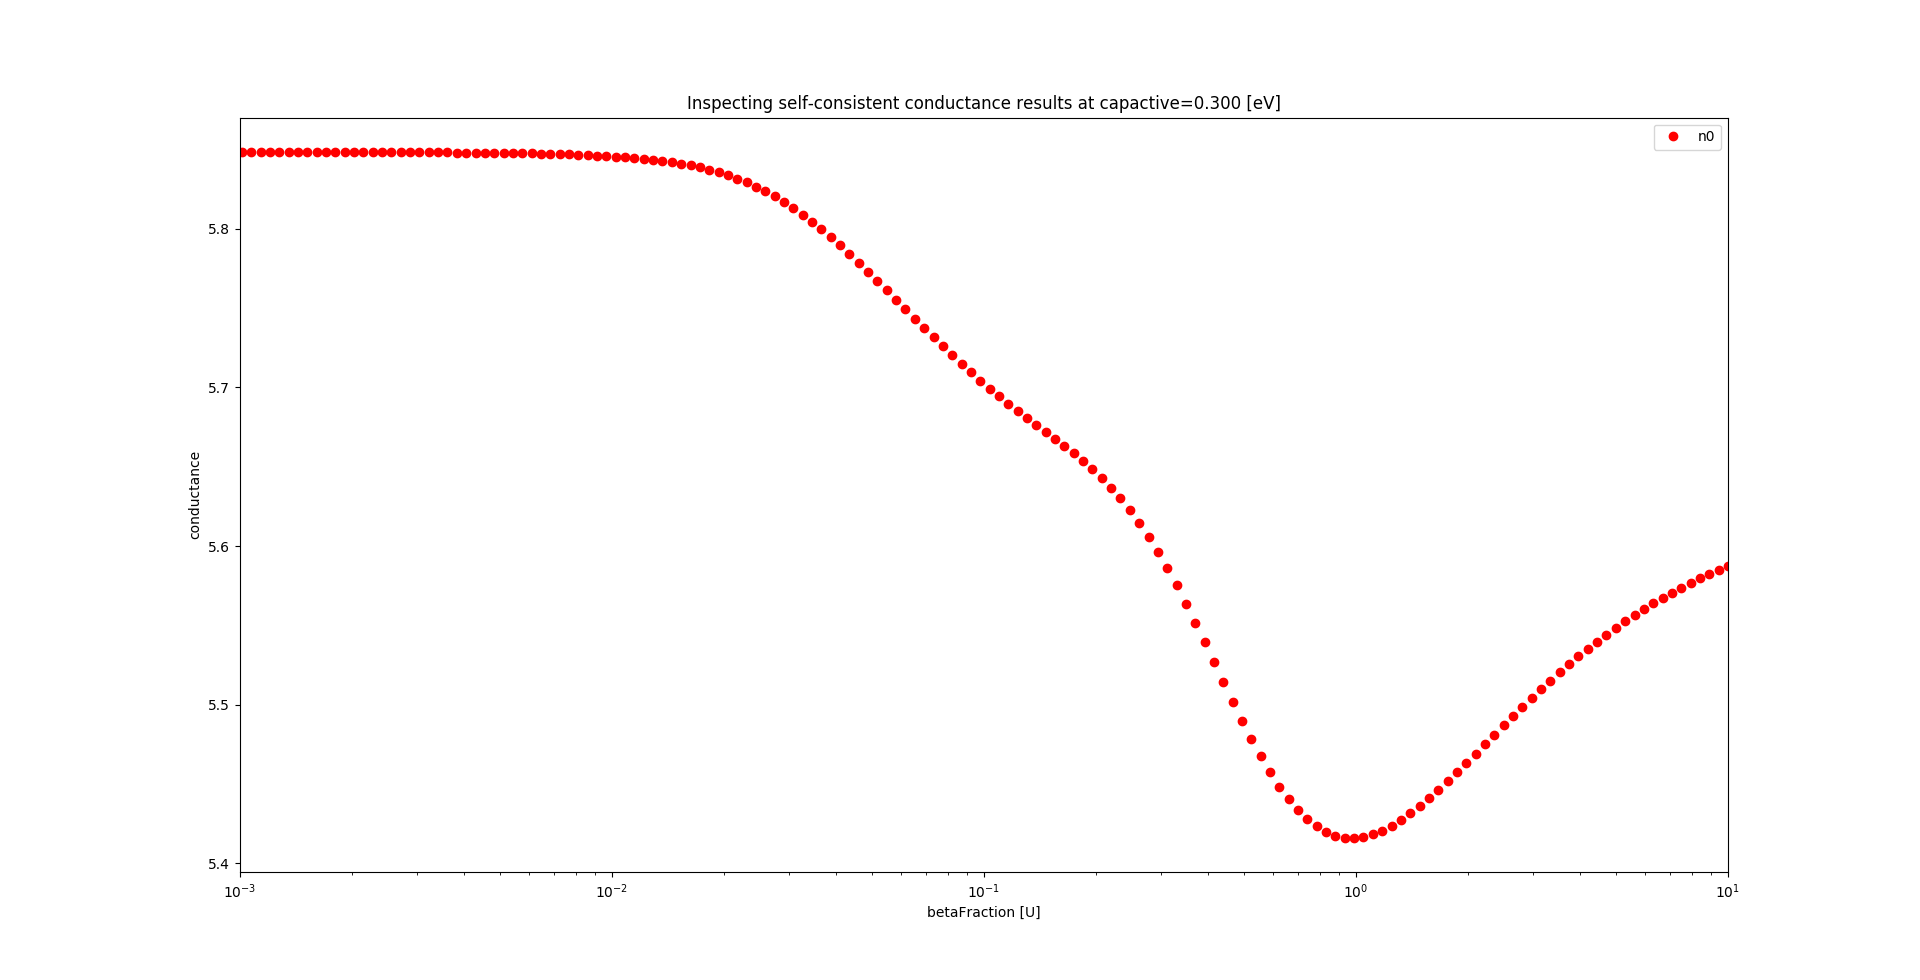
\includegraphics[width=\textwidth]{zeroBiasConductanceLog}
            \caption{\label{fig:conductance} Average of the differential conductance versus temperature. The clear transition from Fermi liquid-like behaviour to logarithmic scaling is evident followed by saturation is evident.}
        \end{figure*}
        
        This indicates that the exact solution is truly exact and incorporates Kondo physics, contrary to many perturbation schemes that are often only valid away from the Kondo temperature $T_K$. Our exact solution thus does not suffer from difficulty in the crossover region. It thus shows excellent agreement with both theory and experiment \cite{Sasaki2000}.
        
        
        
    \section{AH molecule}\label{sec:ahmolecule}
    \section{Discussion}\label{sec:discussion}
    \bibliography{references} 
\end{multicols}
\end{document}
